\documentclass{article}
\usepackage[a4paper, margin=2.5cm]{geometry}
\usepackage{graphicx} % Required for inserting images
\usepackage{pgf} % Required for drawing plots
\usepackage{caption} % Required for the caption of the figure
\usepackage{amsfonts}
\usepackage{xcolor}
\usepackage{amsmath}
\usepackage{amsthm}
\usepackage{hyperref}
\hypersetup{
    colorlinks=true,
    linkcolor=blue,
    filecolor=magenta,
    urlcolor=cyan,
    citecolor=blue
}
\usepackage{cleveref}
\usepackage{enumitem}
\usepackage{float}
\usepackage{diagbox}
\usepackage{caption}
\usepackage{tikz}
\usepackage{pgf}
\usepackage{pgfplots}
\usepackage{placeins} % To use \FloatBarrier
\usetikzlibrary{arrows.meta, positioning}

\newtheorem{theorem}{Theorem}[section]  % Theorems numbered within sections
\newtheorem{lemma}[theorem]{Lemma}      % Lemma numbering follows theorem

% Define argmax
\DeclareMathOperator*{\argmax}{arg\,max}  % The asterisk is used to allow limits to go underneath in displaystyle

% Apply color to cref and Cref
\crefformat{figure}{#2figure\color{blue}~#1#3}
\Crefformat{figure}{#2Figure\color{blue}~#1#3}
\crefformat{section}{#2section\color{blue}~#1#3}
\Crefformat{section}{#2Section\color{blue}~#1#3}
\crefformat{table}{#2table\color{blue}~#1#3}
\Crefformat{table}{#2Table\color{blue}~#1#3}

% start
\title{
    Homework Assignment 4 - Coding Part Write-up\\
    Networks and Markets
}
\author{
    Omer Zohar
    \and
    Gil Aharoni
    \and
    Adam Tuby
}

\bibliographystyle{plain}

\begin{document}
\maketitle

\section*{Part 4: Page Rank and Social Networks}
\setcounter{section}{0}

\section{Question 7}
The two other simple test cases we used are:

\begin{description}
    \item[Extra Graph 1] The first graph is two cycles connected by a single edge (i.e., an infinite loop).
    
    \begin{figure}[H]
        % the tex file at extra_graph_1.tex has \begin{tikzpicture}...\end{tikzpicture}
        \centering
        \resizebox{0.5\textwidth}{!}{%
            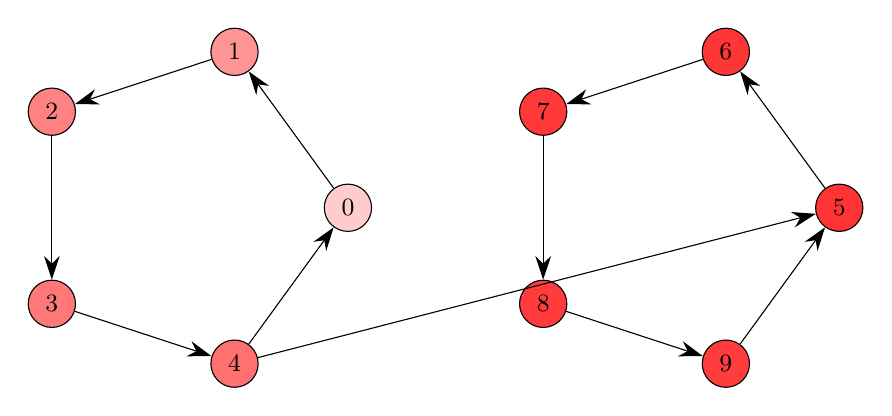
\begin{tikzpicture}[node distance=2cm, every loop/.style={min distance=10mm}]
\node[circle, draw=black, fill=red!20, inner sep=0pt, minimum size=6mm] (node0) at (3.76, 1.98) {\small 0};
\node[circle, draw=black, fill=red!42, inner sep=0pt, minimum size=6mm] (node1) at (2.32, 3.96) {\small 1};
\node[circle, draw=black, fill=red!49, inner sep=0pt, minimum size=6mm] (node2) at (0.00, 3.20) {\small 2};
\node[circle, draw=black, fill=red!53, inner sep=0pt, minimum size=6mm] (node3) at (0.00, 0.76) {\small 3};
\node[circle, draw=black, fill=red!56, inner sep=0pt, minimum size=6mm] (node4) at (2.32, 0.00) {\small 4};
\node[circle, draw=black, fill=red!80, inner sep=0pt, minimum size=6mm] (node5) at (10.00, 1.98) {\small 5};
\node[circle, draw=black, fill=red!79, inner sep=0pt, minimum size=6mm] (node6) at (8.56, 3.96) {\small 6};
\node[circle, draw=black, fill=red!78, inner sep=0pt, minimum size=6mm] (node7) at (6.24, 3.20) {\small 7};
\node[circle, draw=black, fill=red!77, inner sep=0pt, minimum size=6mm] (node8) at (6.24, 0.76) {\small 8};
\node[circle, draw=black, fill=red!76, inner sep=0pt, minimum size=6mm] (node9) at (8.56, 0.00) {\small 9};
\draw[-{Stealth[length=3mm, width=2mm]}] (node0) -- (node1);
\draw[-{Stealth[length=3mm, width=2mm]}] (node1) -- (node2);
\draw[-{Stealth[length=3mm, width=2mm]}] (node2) -- (node3);
\draw[-{Stealth[length=3mm, width=2mm]}] (node3) -- (node4);
\draw[-{Stealth[length=3mm, width=2mm]}] (node4) -- (node0);
\draw[-{Stealth[length=3mm, width=2mm]}] (node4) -- (node5);
\draw[-{Stealth[length=3mm, width=2mm]}] (node5) -- (node6);
\draw[-{Stealth[length=3mm, width=2mm]}] (node6) -- (node7);
\draw[-{Stealth[length=3mm, width=2mm]}] (node7) -- (node8);
\draw[-{Stealth[length=3mm, width=2mm]}] (node8) -- (node9);
\draw[-{Stealth[length=3mm, width=2mm]}] (node9) -- (node5);
\end{tikzpicture}

        }
        \caption{Extra Graph 1}
    \end{figure}

    \item[Extra Graph 2] The second graph is a bipartite graph with 5 nodes on each side, where each node on one side is connected to all nodes on the other side.
    
    \begin{figure}[H]
        % the tex file at extra_graph_2.tex has \begin{tikzpicture}...\end{tikzpicture}
        \centering
        \resizebox{0.4\textwidth}{!}{%
            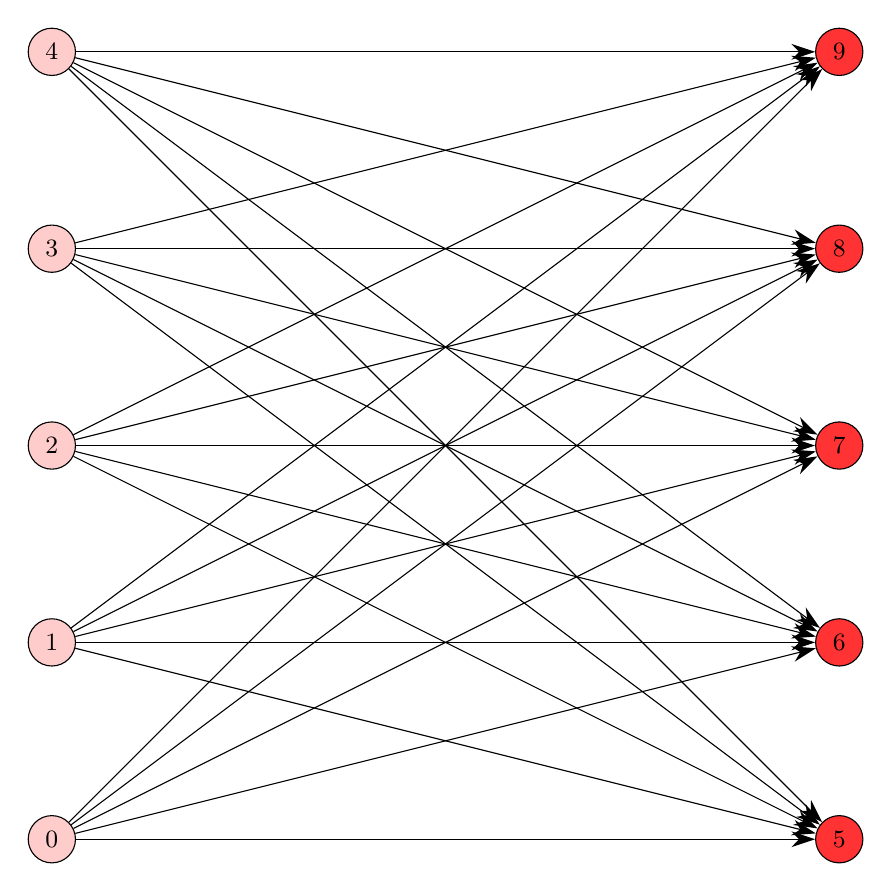
\begin{tikzpicture}[node distance=2cm, every loop/.style={min distance=10mm}]
\node[circle, draw=black, fill=red!20, inner sep=0pt, minimum size=6mm] (node0) at (0.00, 0.00) {\small 0};
\node[circle, draw=black, fill=red!20, inner sep=0pt, minimum size=6mm] (node1) at (0.00, 2.50) {\small 1};
\node[circle, draw=black, fill=red!20, inner sep=0pt, minimum size=6mm] (node2) at (0.00, 5.00) {\small 2};
\node[circle, draw=black, fill=red!20, inner sep=0pt, minimum size=6mm] (node3) at (0.00, 7.50) {\small 3};
\node[circle, draw=black, fill=red!20, inner sep=0pt, minimum size=6mm] (node4) at (0.00, 10.00) {\small 4};
\node[circle, draw=black, fill=red!80, inner sep=0pt, minimum size=6mm] (node5) at (10.00, 0.00) {\small 5};
\node[circle, draw=black, fill=red!80, inner sep=0pt, minimum size=6mm] (node6) at (10.00, 2.50) {\small 6};
\node[circle, draw=black, fill=red!80, inner sep=0pt, minimum size=6mm] (node7) at (10.00, 5.00) {\small 7};
\node[circle, draw=black, fill=red!80, inner sep=0pt, minimum size=6mm] (node8) at (10.00, 7.50) {\small 8};
\node[circle, draw=black, fill=red!80, inner sep=0pt, minimum size=6mm] (node9) at (10.00, 10.00) {\small 9};
\draw[-{Stealth[length=3mm, width=2mm]}] (node0) -- (node5);
\draw[-{Stealth[length=3mm, width=2mm]}] (node0) -- (node6);
\draw[-{Stealth[length=3mm, width=2mm]}] (node0) -- (node7);
\draw[-{Stealth[length=3mm, width=2mm]}] (node0) -- (node8);
\draw[-{Stealth[length=3mm, width=2mm]}] (node0) -- (node9);
\draw[-{Stealth[length=3mm, width=2mm]}] (node1) -- (node5);
\draw[-{Stealth[length=3mm, width=2mm]}] (node1) -- (node6);
\draw[-{Stealth[length=3mm, width=2mm]}] (node1) -- (node7);
\draw[-{Stealth[length=3mm, width=2mm]}] (node1) -- (node8);
\draw[-{Stealth[length=3mm, width=2mm]}] (node1) -- (node9);
\draw[-{Stealth[length=3mm, width=2mm]}] (node2) -- (node5);
\draw[-{Stealth[length=3mm, width=2mm]}] (node2) -- (node6);
\draw[-{Stealth[length=3mm, width=2mm]}] (node2) -- (node7);
\draw[-{Stealth[length=3mm, width=2mm]}] (node2) -- (node8);
\draw[-{Stealth[length=3mm, width=2mm]}] (node2) -- (node9);
\draw[-{Stealth[length=3mm, width=2mm]}] (node3) -- (node5);
\draw[-{Stealth[length=3mm, width=2mm]}] (node3) -- (node6);
\draw[-{Stealth[length=3mm, width=2mm]}] (node3) -- (node7);
\draw[-{Stealth[length=3mm, width=2mm]}] (node3) -- (node8);
\draw[-{Stealth[length=3mm, width=2mm]}] (node3) -- (node9);
\draw[-{Stealth[length=3mm, width=2mm]}] (node4) -- (node5);
\draw[-{Stealth[length=3mm, width=2mm]}] (node4) -- (node6);
\draw[-{Stealth[length=3mm, width=2mm]}] (node4) -- (node7);
\draw[-{Stealth[length=3mm, width=2mm]}] (node4) -- (node8);
\draw[-{Stealth[length=3mm, width=2mm]}] (node4) -- (node9);
\end{tikzpicture}

        }
        \caption{Extra Graph 2}
    \end{figure}
\end{description}

\section{Question 8}

\begin{enumerate}

    \item[(c)] Running PageRank on the given graph, we get that nodes with high ranks typically have higher degrees, and nodes with low ranks typically have lower degrees.\\
    The top 5 nodes with the highest page rank had the following degrees: 547, 1045, 792, 347, 755 (where top rank had 547 neighbors, and 5th had 755).\\
    The bottom 5 nodes with the lowest page rank had the following degrees: 1, 1, 1, 1, 1.\\

    \item[(d)] Intuitively, the page rank of a node is the probability that a random walker will be at that node at a given time.\\
    If a node has a high rank, then starting a random walk from many nodes it is likely to arrive at that node.\\
    Since the graph is equivalent to an undirected one, it means that a high rank means that random walks from it might reach many nodes.\\
    If we want to quantify influence over people using it, it seems that the scaled page rank is a good measure.\\

\end{enumerate}

\end{document}